\subsection{Unsupervised Learning}
There were no unsupervised methods that provided obvious structure  that matched the classifications.  For the K-means method, a variety of k-values were used.  In each case, the positive cases were divided among the categories in rough proportion to the total number of cases in each category.  A similar thing happened with LDA.  Since LDA is a mixed membership model, we decided to assign hard membership if an object had larger than a certain threshold (e.g., 0.8 or 0.9) membership in a particular topic.  Members of a particular topic were distributed between positive and negative examples in rough proportion to the actual distributions of the examples in the data set.  GMM, for small values of \texttt{n\_components}, was able to do better than just randomly pulling from the dataset for its category assignment.  For example, for \texttt{n\_components} = 4, one of the categories (using a posterior probability threshold of 0.9) had ${\sim}$25\% of its members being positive examples and another category had only ${\sim}$0.1\% of its members being positive examples.  If the GMM category assignment was nothing more than random draws from the data, then both of these percentages would be around 3.3\%.  (The other two categories have ${\sim}$1--2\% of their members being positive examples).  Thus, GMM was able to uncover some features in the data that allowed for a small differentiation between positive and negative examples.  Unfortunately, only ${\sim}$10\% of the positive examples end up in the positive-heavy category, which itself still consists ${\sim}$75\% of negative examples, so the GMM categories themselves are not sufficiently discriminatory to be used as our model.

For PCA, the first principal component explains 20\% of the variance, then 11\%, 8.5\%, and 7.8\% for the next three principal components.  Figure~\ref{pca} shows the projection of the data onto the first two principal components.  The green circles are the positive cases and blue dots are the negative cases.  Although the variance between the two sets of points is different (22.6 along the first principal component for the green points versus 17.7 for the blue), from just the first two principal components there is no exploitable separation between the positive and negative cases that allows for classification.  Running K-means (with several different values of k) on the PCA-decomposed values also revelead no exploitable structure for classification.  Running GMM on the PCA-decomposed values provided clustering with worse predictive power than GMM on the normal data (the ``best'' cluster only had ${\sim}$13\% of its members being positive cases, instead of ${\sim}$25\% as was the case before).
\begin{figure}
\begin{centering}
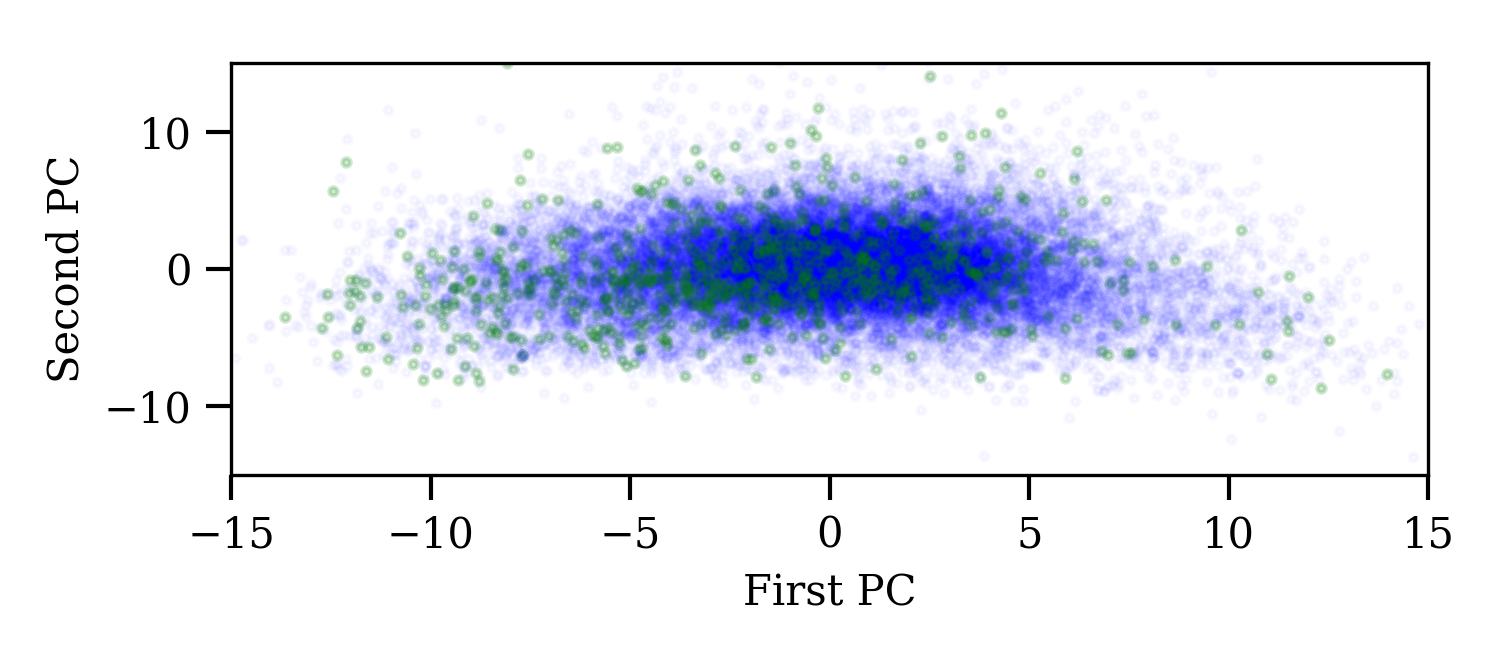
\includegraphics[width=5in]{pca.png}
\caption{\label{pca} The data projected on the first two principal components.  The positive cases are in green and the negative cases are in blue.  Note that the scales of the axes are the same; they have been stretched and squished to better fit in the single-column format of this paper.  The transparency of the green points is less than the blue points so that they could be better visible, since there are about 30 times more blue points than green points.  There is no obvious separation between the two groups of points, though the green points do have larger variance than the blue points along the first principal component (22.6 versus 17.7).  In the axis labels, ``PC'' = principal component.}
\end{centering}
\end{figure}







\subsection{Supervised Learning}

We focused on four metrics to assess our models. These were the precision, recall, negative predictive value (NPV; the ``precision'' of the negative cases), and specificity (the ``recall'' of the negative cases).  It should be noted that our data set is very imbalanced, with many more negative cases (29,420) than positive cases (1024). The result of this was that for almost all of estimators we achieved high NPV and specificity, thus the more interesting metrics are the precision and recall.  Also, since we care more about the accuracy positive cases (these are what go on to hopefully be planet discoveries after all), precision and recall are more important than NPV and specificity (although the values of each are related to each other).

In table \ref{table:classifiers} we present the average precision and recall of our classifiers on the with-held data set averaged from $25$ fold cross-validation. The results show that the best methods are the Naive Bayes and Gradient Boosting method . In table \ref{table:votingClassifiers} we show the results of combining our classifiers and using soft and hard voting methods. We found that we achieved the best results in this method by only using the best two classifiers rather than all of the classifiers however this was not an improvement on the separate classifiers.

\begin{table}
 \begin{tabular}{|l |l |l |l |l |}
\hline
Classifier &NPV & Specificity &Precision & Recall  \\ \hline
 NaiveBayes & 0.984 &  0.967&  0.369 & 0.555 \\ 
GradientBoosting & 0.979 & 0.992 &  0.628 & 0.386\\
RandomForest & 0.975 &  0.988 & 0.429&  0.263 \\
ExtraTrees & 0.974 & 0.987 &  0.407& 0.252 \\
AdaBoost & 0.973&  0.992 & 0.502& 0.202 \\
%SVM & & & & \\
LogisticReg &0.969 &  0.995& 0.3767 &  0.080\\\hline
\end{tabular}
\caption{Class 0 -not selected, Class 1 selected}
\label{table:classifiers}
\end{table}

\begin{table}
 \begin{tabular}{|l |l |l |l |l |}
\hline
Classifier &Precision - class 0 & Recall - class 0  &Precision - class 1 & Recall - class 1  \\ \hline
All classifiers - Hard & 0.969&  0.995&  0.368&  0.077\\
All classifiers  - Soft & 0.969 &  0.995&  0.365&   0.074\\ 
Best Two - Hard & 0.979&  0.992&  0.634&  0.383\\
Best Two  - Soft &0.978&  0.992 & 0.612 &  0.373\\ \hline
\end{tabular}
\caption{Class 0 -not selected, Class 1 selected}
\label{table:votingClassifiers}
\end{table}
